
\section{Definição de Arquitetura de Software}
A arquitetura de software possibilita entender as diferenças entre as linguagens, sistemas operativos, ou seja, qualquer componente tecnológico pode ser usado para integrar uma solução de arquitetura de software. É essencial pois otimiza o trabalho dos designers e programadores, permitindo que uma aplicação esteja dentro dos padrões básicos necessários para funcionar de forma assertiva.\\*
A Arquitetura de Software é importante para automatizar novos processos ou melhorar os já existentes, mas para isso envolve:
\begin{itemize}
    \item Decisões sobre as estruturas do sistema;
    \item Controlo;
    \item Protocolos de comunicação, sincronização e acesso a dados;
    \item Desempenho e outros atributos de qualidade.
\end{itemize}

Implementar uma arquitetura de software traz diversos benefícios para o sistema. Entre eles, os três principais são:
\begin{itemize}
    \item Performance;
    \item Escalabilidade;
    \item Flexibilidade.
\end{itemize}


\section{Evolução das Aplicações Web}
O desenvolvimento web, a par de outras áreas tecnológicas, está em constante evolução. O que vemos hoje não é o mesmo que víamos à 10 anos atrás e a prova disso são as aplicações que usamos hoje. Como consequência o acesso à informação digital também mudou drasticamente. Agora são os dispositivos móveis a serem a opção preferida para aceder à informação. A grande evolução das aplicações web na minha opinião foi devido ao avanço e à quantidade de dispositivos móveis. Ainda hoje estamos perante mudanças a "toda a hora" por causa dos dispositivos móveis, quer seja a nível de qualidade ou desempenho.

Com a imagem seguinte podemos verificar o avanço das tecnologias em função do tempo. Verificamos que começamos a ter um grande avanço com a tecnologia \textit{Web 2.0} e mais recentemente a recém chegada \textit{Web 3.0}. 

\begin{figure}[H]
\center
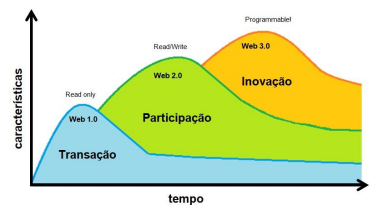
\includegraphics[width=12cm]{web.png}
\caption{Evolução das tecnologias Web}
\end{figure}



\section{Arquiteturas mais Populares}
Alguns exemplos das arquiteturas mais populares:
\begin{itemize}
    \item Layers (Camadas)
    \item Client-Server (Cliente-Servidor)
    \item \ac{MVC}
    \item \ac{P2P}
    \item Microservices (Micro serviços)
\end{itemize}

A arquitetura em camadas, como o nome indica, é organizada num conjunto de camadas, oferecendo maior flexibilidade e suporte a portabilidade. A identificação do nível de abstração nem sempre é evidente e perde-se desempenho à medida que o número de camadas cresce. Um exemplo onde é aplicado esta arquitetura é nas aplicações \textit{E-Commerce}.\\*
\indent Na arquitetura Cliente-Servidor o processamento da informação divide-se em módulos e processos distintos, sendo um deles responsável pela manutenção da informação e o outro pela obtenção de dados. Um exemplo do seu uso é no serviço de \textit{e-mail}.\\*
\indent A arquitetura \ac{MVC} é uma referência para nós (estudantes), uma vez que é uma arquitetura lecionada na disciplina de \ac{PWEB}. O sistema \ac{MVC} separa o projeto do software em três camadas independentes: o modelo/model (manipulação lógica de dados), a visão/view (interface do usuário) e o controlador/controller (fluxo de aplicação), facilitando a manutenção do código, que pode ser reutilizado em outros projetos.\\*
\indent Passando ao \ac{P2P}, todos os pares são clientes e servidores, ou seja, cada computador é um provedor de serviços independente de um servidor central. \textit{Torrent}, a aplicação tão conhecida por nós onde usa esta arquiterura.\\*
\indent Em último, e não menos importante, temos a arquitetura Microservices onde se baseia em múltiplos serviços e componentes para desenvolver uma estrutura modular. É o padrão mais utilizado por \textit{devs} e engenheiros(as) de software, por permitir escalabilidade e independência dos módulos, que podem usar diferentes linguagens.


\section{Arquitetura de Aplicações Web}
A arquitetura de aplicações Web é o ponto de partida  para desenvolver uma aplicação. No entanto, existem vários aspetos de implementação. Por exemplo, como etapa inicial, a escolha de uma linguagem de programação para desenvolver a aplicação.

Existe uma panóplia de linguagens de programação usadas no desenvolvimento de software. Algumas delas utilizadas na criação de determinados tipos de aplicações, como \textit{Swift}, \textit{Java}, para aplicações mobile ou \textit{JavaScript} para desenvolvimento \textit{front-end}.


\subsection{Tipos de Arquitetura de Aplicações Web}
\begin{itemize}
    \item \ac{SOA}
    \item Microservices (micro serviços)
\end{itemize}
